
\subsection{Ladestation} \label{sec:ladestation}

Nachdem die gesamte induktive Ladeschaltung beschrieben wurde, folgt die Beschreibung der Ladestation. Hierfür wurde ein Prototyp erstellt, welche zum einen die gesamte primäre induktive Ladeschaltung beinhaltet, zum anderen eine Aussparung, welche als Ladeeinrichtung für den Dōjō dient, vorweist. Für den Prototypen wurde eine .stl Datei erstellt welche mit einem 3D-Drucker gedruckt wurde. Wichtig ist hierbei zu erwähnen, dass es sich bei nachfolgende Abbildungen \ref{fig:Prototyp Front} bis \ref{fig:Prototyp Down} nur um Prototypen handelt und es bei einer Weiterentwicklung noch Anpassungen geben kann. Da die Ladestation für Versuchszwecke betreffend der induktiven Ladeschaltung bereits erstellt wurde, ist das Design so gewählt, dass nur ein Dōjō geladen werden kann. Dies könnte in einem weiteren Schritt auf mehrere Ladeaussparungen erweitert werden, wobei mehrere Dōjōs gleichzeitig pro Ladestation geladen werden können. 

\begin{figure}[H]
	\begin{center}
		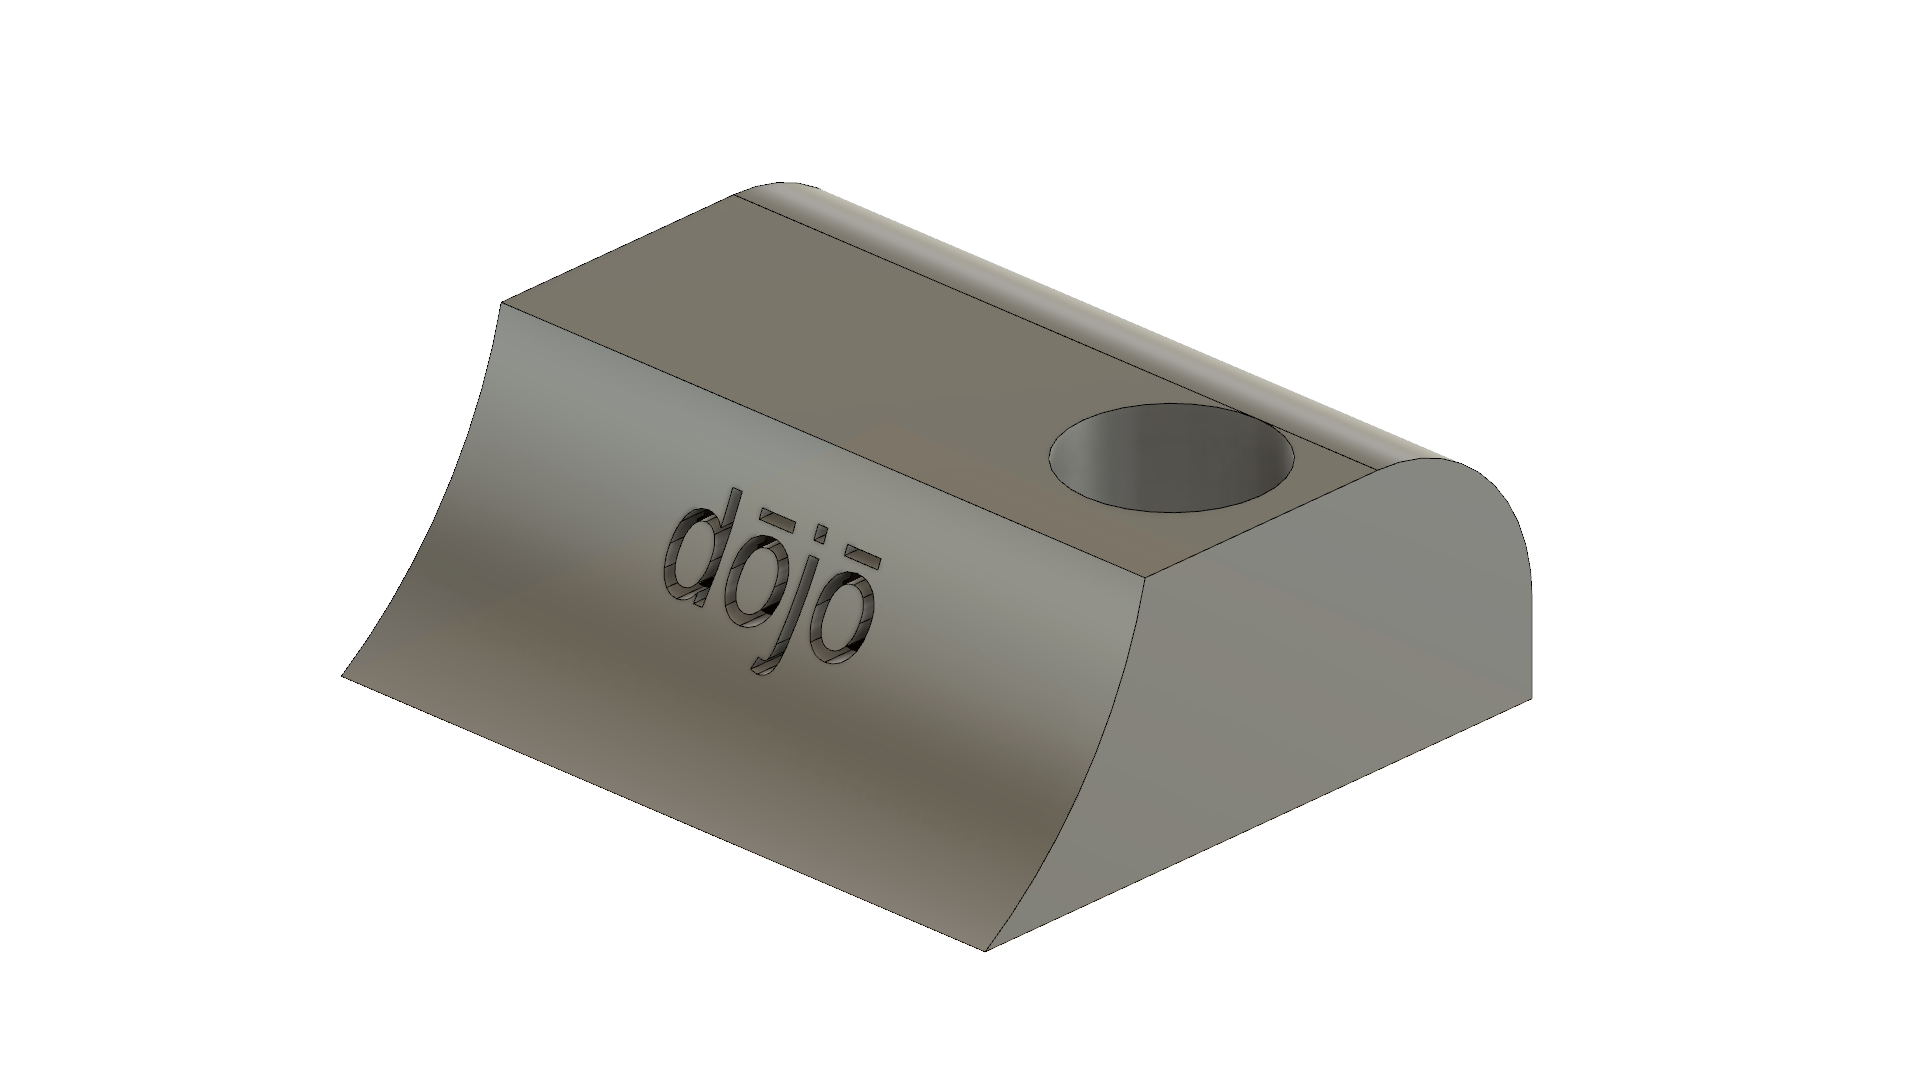
\includegraphics[width=80mm]{data/DojoLadestation01.png}
		\caption[Prototyp Ladestation Frontansicht]{Frontansicht - Ladestation Dōjō} %picture caption
		\label{fig:Prototyp Front}
	\end{center}
\end{figure}

Die oben gezeigte Abbildung gibt einen Einblick in das Design von vorne. Augenfällig ist die Öffnung für den Dōjō selbst, welche zum einen als Standhalterung und zum anderen als korrekte Positionierung für die induktive Ladeschaltung dient. Die richtige Positionierung ist hierbei eines der wichtigsten Kriterien für einen optimalen Ladezyklus, da die Tranceiver- und Receiverspule direkt übereinanderliegend den besten Wirkungsgrad erzielen. Weiter ist in der Abbildung der Dōjō Schriftzug ersichtlich, welcher bis in die dahinter liegende Kammer führt. Die Verwendung dieser Durchführung wird nachfolgend unter der Abbildung \ref{fig:Prototyp Down} weiter erklärt. 


\begin{figure}[H]
	\begin{center}
		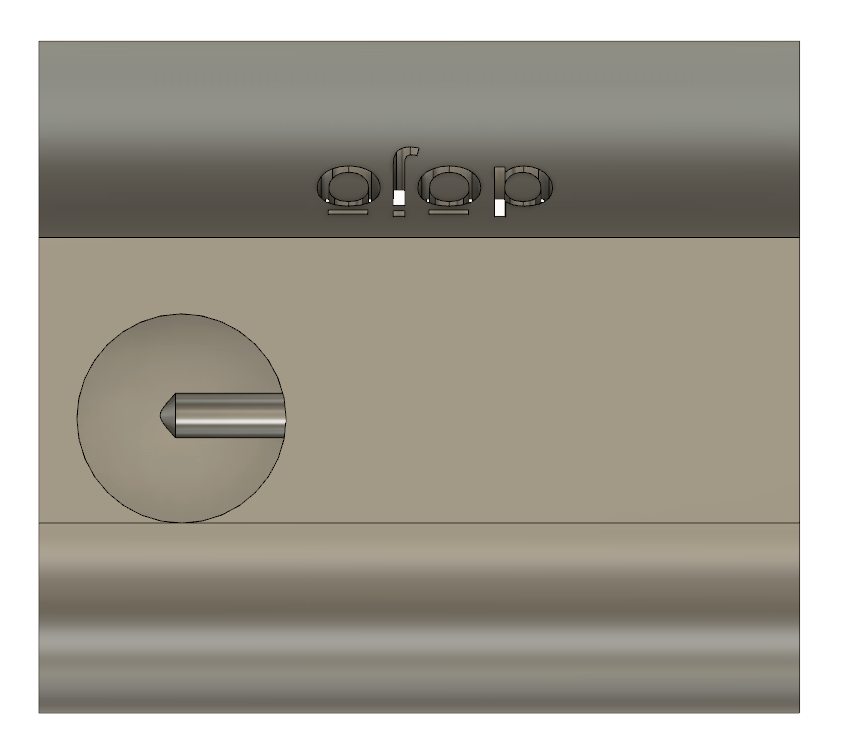
\includegraphics[width=80mm]{data/DojoLadestation02.png}
		\caption[Prototyp Ladestation Draufsicht]{Draufsicht - Ladestation Dōjō} %picture caption
		\label{fig:Prototyp Top}
	\end{center}
\end{figure}

Die obige Abbildung \real{fig: Prototyp Top} zeigt den Prototypen von oben. In der Aussparung für den Dōjō ist ein Kanal für die Verkabelung der Primärspule ersichtlich. Diese Öffnung führt zur Kammer welche den Primär-Ladekreises beinhaltet. Die Abmessung (Länge x Breite x Höhe) des Prototypen ist (80 x 70.7 x 30)mm. Einen Einblick in die Kammer für die Elektronik des Primär-Ladekreises gibt nachfolgende Abbildung \ref{fig:Prototyp Down}, welche den Prototypen von unten zeigt.

\begin{figure}[H]
	\begin{center}
		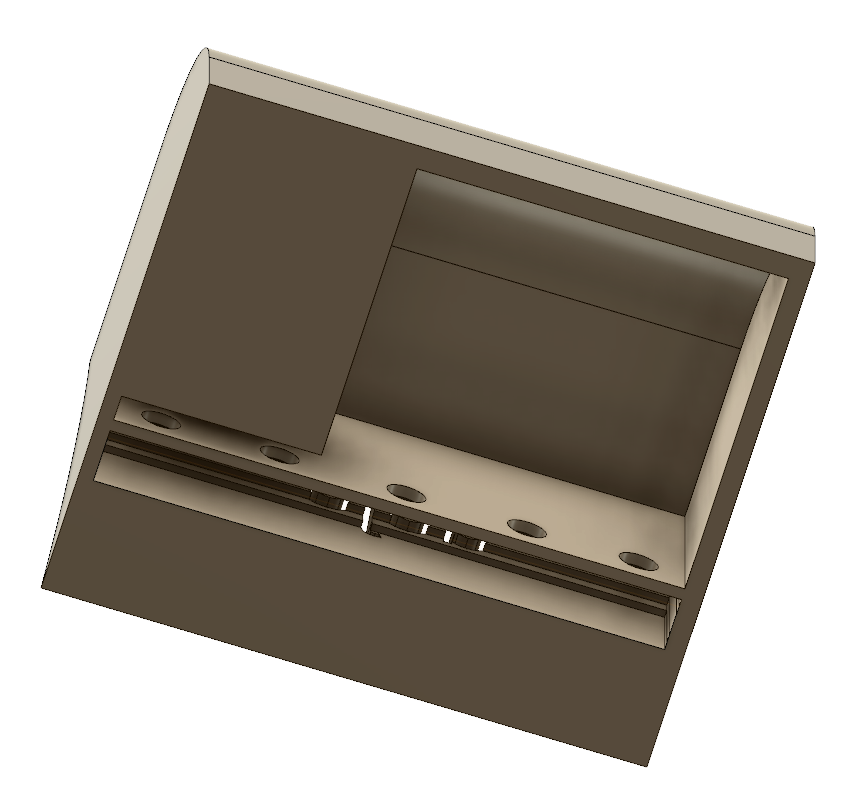
\includegraphics[width=80mm]{data/DojoLadestation03.png}
		\caption[Prototyp Ladestation Ansicht von Unten]{Ansicht von Unten - Ladestation Dōjō} %picture caption
		\label{fig:Prototyp Down}
	\end{center}
\end{figure}

Die grosse Kammer ist wie bereits oben beschrieben für den Primärkreis der induktiven Ladeschaltung vorgesehen. Für die ersten Tests wurde eine Lochrasterplatine mit allen nötigen Komponenten gefertigt, welche genau in diese Aussparung passt. Weiter sind runde Löcher (5mm $\o$) ersichtlich welche in die Kammer des Schriftzuges führen ersichtlich. Diese Durchführungen sind für LED vorgesehen, welche den Dōjō Schriftzug bei angeschlossener Versorgungsspannung zum Leuchten bringt. 